\documentclass{article}

\usepackage{fancyhdr}
\usepackage{extramarks}
\usepackage{amsmath}
\usepackage{amsthm}
\usepackage{amsfonts}
\usepackage{tikz}
\usepackage[plain]{algorithm}
\usepackage{algpseudocode}
\usepackage{graphicx}
\usepackage{epstopdf}
\usepackage{xfrac}
\usepackage{siunitx}
\usepackage[americanvoltages]{circuitikz}
\usepackage{booktabs}

\usetikzlibrary{automata,positioning}

%
% Basic Document Settings
%

\topmargin=-0.45in
\evensidemargin=0in
\oddsidemargin=0in
\textwidth=6.5in
\textheight=9.0in
\headsep=0.25in

\linespread{1.1}

\pagestyle{fancy}
\lhead{\hmwkAuthorName}
\chead{\hmwkClass\ (\hmwkClassInstructor\ \hmwkClassTime): \hmwkTitle}
\rhead{\firstxmark}
\lfoot{\lastxmark}
\cfoot{\thepage}

\renewcommand\headrulewidth{0.4pt}
\renewcommand\footrulewidth{0.4pt}

\setlength\parindent{0pt}

%
% Create Problem Sections
%

\newcommand{\enterProblemHeader}[1]{
    \nobreak\extramarks{}{Problem \arabic{#1} continued on next page\ldots}\nobreak{}
    \nobreak\extramarks{Problem \arabic{#1} (continued)}{Problem \arabic{#1} continued on next page\ldots}\nobreak{}
}

\newcommand{\exitProblemHeader}[1]{
    \nobreak\extramarks{Problem \arabic{#1} (continued)}{Problem \arabic{#1} continued on next page\ldots}\nobreak{}
    \stepcounter{#1}
    \nobreak\extramarks{Problem \arabic{#1}}{}\nobreak{}
}

\setcounter{secnumdepth}{0}
\newcounter{partCounter}
\newcounter{homeworkProblemCounter}
\setcounter{homeworkProblemCounter}{1}
\nobreak\extramarks{Problem \arabic{homeworkProblemCounter}}{}\nobreak{}

%
% Homework Problem Environment
%
% This environment takes an optional argument. When given, it will adjust the
% problem counter. This is useful for when the problems given for your
% assignment aren't sequential. See the last 3 problems of this template for an
% example.
%
\newenvironment{homeworkProblem}[1][-1]{
    \ifnum#1>0
        \setcounter{homeworkProblemCounter}{#1}
    \fi
    \section{Problem \arabic{homeworkProblemCounter}}
    \setcounter{partCounter}{1}
    \enterProblemHeader{homeworkProblemCounter}
}{
    \exitProblemHeader{homeworkProblemCounter}
}

%
% Homework Details
%   - Title
%   - Due date
%   - Class
%   - Section/Time
%   - Instructor
%   - Author
%

\newcommand{\hmwkTitle}{Assignment\ 3}
\newcommand{\hmwkDueDate}{June 3, 2017}
\newcommand{\hmwkClass}{Power Systems Analysis}
\newcommand{\hmwkClassTime}{}
\newcommand{\hmwkClassInstructor}{Kamal Debnath}
\newcommand{\hmwkAuthorName}{S.Reynolds (262538)}

%
% Title Page
%

\title{
    \vspace{2in}
    \textmd{\textbf{\hmwkClass:\ \hmwkTitle}}\\
    \normalsize\vspace{0.1in}\small{Due\ on\ \hmwkDueDate\ at 3:00pm}\\
    \vspace{0.1in}\large{\textit{\hmwkClassInstructor\ \hmwkClassTime}}
    \vspace{3in}
}

\author{\textbf{\hmwkAuthorName}}
\date{}

\renewcommand{\part}[1]{\textbf{\large Part \Alph{partCounter}}\stepcounter{partCounter}\\}

%
% Various Helper Commands
%

% Useful for algorithms
\newcommand{\alg}[1]{\textsc{\bfseries \footnotesize #1}}

% For derivatives
\newcommand{\deriv}[1]{\frac{\mathrm{d}}{\mathrm{d}x} (#1)}

% For partial derivatives
\newcommand{\pderiv}[2]{\frac{\partial}{\partial #1} (#2)}

% Integral dx
\newcommand{\dx}{\mathrm{d}x}

% Alias for the Solution section header
\newcommand{\solution}{\textbf{\large Solution}}

% Probability commands: Expectation, Variance, Covariance, Bias
\newcommand{\E}{\mathrm{E}}
\newcommand{\Var}{\mathrm{Var}}
\newcommand{\Cov}{\mathrm{Cov}}
\newcommand{\Bias}{\mathrm{Bias}}

\graphicspath{{./fig/}}

\begin{document}

\maketitle

\pagebreak

Consider the power system shown in Figure 1. Each three phase transformer is made up of three single phase transformers. The squares $B_1$, $B_2$, $B_3$,...,$B_6$ are circuit breakers which can be considered to have very low series impedance while closed and infinite impedance when open.

\begin{figure}[H]
	\centering
	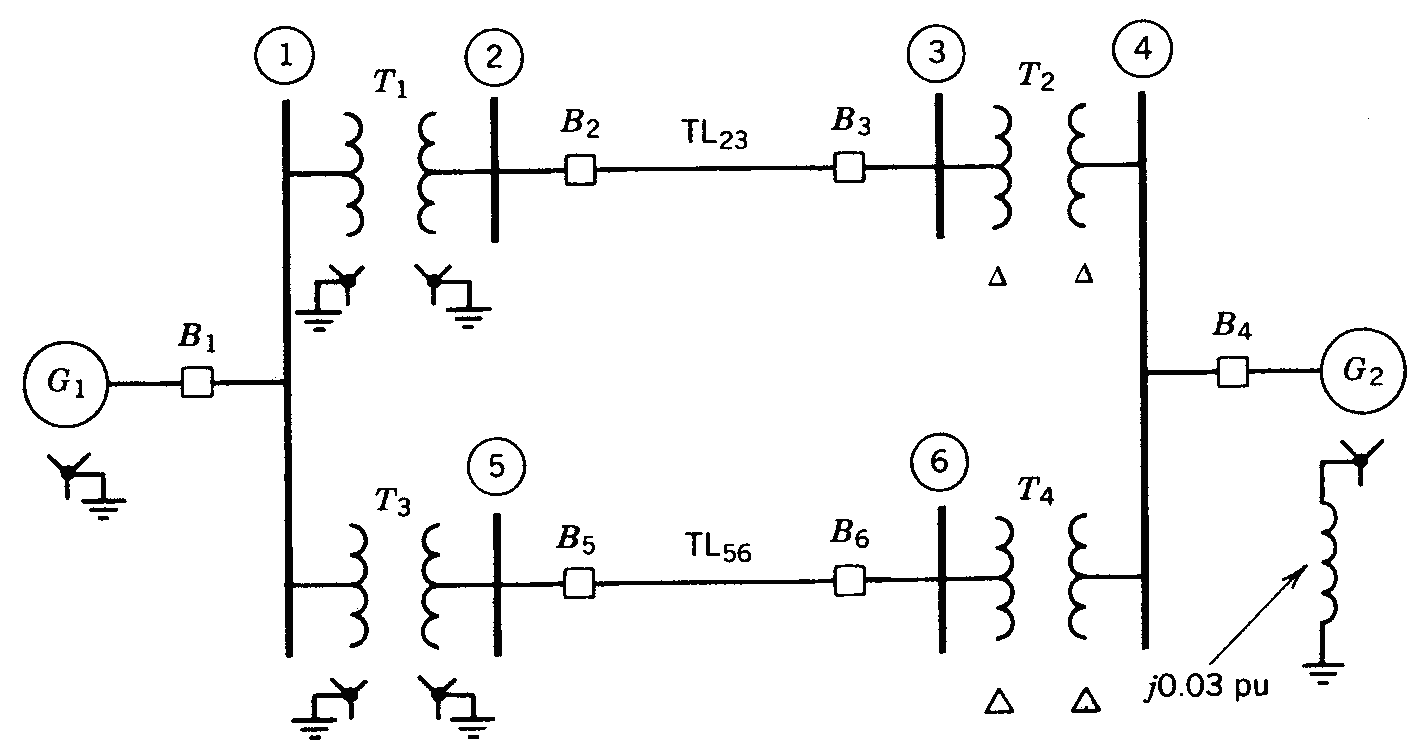
\includegraphics[scale=0.3]{fig1}
	\caption{text}
\end{figure}

\begin{figure}[H]
	\centering
	\caption{text}
	\begin{tabular}{crrrrr}
		\toprule
		\textbf{Component}	&	\textbf{Power Rating}	&	\textbf{Voltage Rating}	&	$X_1$	& 	$X_2$	&	$X_0$\\
					&	(MVA)			&	(kV)			&	(pu)	&	(pu)	&	(pu)\\
		\midrule
		$G_1$		&	200				&	20				&	0.2		&	0.14	&	0.06\\
		$G_2$		&	200				&	13.2			&	0.2		&	0.14	&	0.06\\
		$T_1$		&	200				&	20/230			&	0.2		&	0.2		&	0.2\\
		$T_2$		&	200				&	13.2/230		&	0.3		&	0.3		&	0.3\\
		$T_3$		&	200				&	20/230			&	0.25	&	0.25	&	0.25\\
		$T_4$		&	200				&	13.2/230		&	0.35	&	0.35	&	0.35\\
		$TL_{23}$	&	200				&	230				&	0.15	&	0.15	&	0.3\\
		$TL_{56}$	&	200				&	230				&	0.22	&	0.22	&	0.5\\
		\bottomrule	
	\end{tabular}
\end{figure}

\section{Assignment 3.1 - PART A}
The following section details the three sequence networks, and the impedance vlued

\subsection{Zero Sequence Network}

\begin{figure}[H]
	\centering
	\begin{circuitikz}
		\draw
		(0,2) node[label={[font=\footnotesize]above:$1$}]{}
		to [L,l=$j0.2$,-*] (2,2) node[label={[font=\footnotesize]above:$2$}]{}
		to [L,l=$j0.3$,-o] (4,2) node[label={[font=\footnotesize]above:$3$}]{}
		;
		
		\draw
		(0,0) node[]{}
		to [L,l=$j0.2$,-*] (2,0) node[label={[font=\footnotesize]above:$5$}]{}
		to [L,l=$j0.3$,-o] (4,0) node[label={[font=\footnotesize]above:$6$}]{}
		;
		
		\draw (0,0) -- (0,2);
		
		\draw (-2,1)
		to [L,l=$j0.06$,] (0,1)
		;
		
		\draw (-2,1) -- (-2,0) node[ground]{};
		
		\draw (5,2)
		to [L,l=$j0.3$] (7,2)
		;
		\draw (5,2) -- (5,1.5) node[ground]{};
		\draw (7,2) -- (7,1.5) node[ground]{};
		
		\draw (5,0)
		to [L,l=$j0.35$] (7,0)
		;
		\draw (5,0) -- (5,-0.5) node[ground]{};
		\draw (7,0) -- (7,-0.5) node[ground]{};
		
		\draw (8,2)
		to [short,o-] (9,2) node[label={[font=\footnotesize]above:$4$}]{}
		;
		
		\draw (8,0)
		to [short,o-] (9,0)
		;
		
		\draw (9,2) -- (9,0);
		
		\draw (9,1)
		to [L,l=$j0.06$] (11,1)
		to [L,l=$j0.09$] (13,1)
		;
		
		\draw (13,1) -- (13,0) node[ground]{};
	\end{circuitikz}
\end{figure}

\subsection{Positive Sequence Network}

\begin{figure}[H]
	\centering
	\begin{circuitikz}
		\draw
		(0,2) node[label={[font=\footnotesize]above:$1$}]{}
		to [L,l=$j0.2$,-*] (2,2) node[label={[font=\footnotesize]above:$2$}]{}
		to [L,l=$j0.15$,-*] (4,2) node[label={[font=\footnotesize]above:$3$}]{}
		to [L,l=$j0.3$] (6,2) node[label={[font=\footnotesize]above:$4$}]{}
		;
		
		\draw
		(0,0) node[]{}
		to [L,l=$j0.25$,-*] (2,0) node[label={[font=\footnotesize]above:$5$}]{}
		to [L,l=$j0.22$,-*] (4,0) node[label={[font=\footnotesize]above:$6$}]{}
		to [L,l=$j0.35$] (6,0)
		;
		
		\draw (0,0) -- (0,2);
		
		\draw (-2,-1)
		to [sV] (-2,1)
		to [L,l=$j0.2$,] (0,1)
		;
		
		\draw (-2,-1) -- (-2,-1) node[ground]{};
		
		\draw (6,2) -- (6,0);
		
		\draw (6,1)
		to [L,l=$j0.2$] (8,1)
		to [sV] (8,-1)
		;
		
		\draw (8,-1) -- (8,-1) node[ground]{};
	\end{circuitikz}
\end{figure}


\subsection{Negative Sequence Network}

\begin{figure}[H]
	\centering
	\begin{circuitikz}
		\draw
		(0,2) node[label={[font=\footnotesize]above:$1$}]{}
		to [L,l=$j0.2$,-*] (2,2) node[label={[font=\footnotesize]above:$2$}]{}
		to [L,l=$j0.15$,-*] (4,2) node[label={[font=\footnotesize]above:$3$}]{}
		to [L,l=$j0.3$] (6,2) node[label={[font=\footnotesize]above:$4$}]{}
		;
		
		\draw
		(0,0) node[]{}
		to [L,l=$j0.25$,-*] (2,0) node[label={[font=\footnotesize]above:$5$}]{}
		to [L,l=$j0.22$,-*] (4,0) node[label={[font=\footnotesize]above:$6$}]{}
		to [L,l=$j0.35$] (6,0)
		;
		
		\draw (0,0) -- (0,2);
		
		\draw (-2,1)
		to [L,l=$j0.06$,] (0,1)
		;
		
		\draw (-2,1) -- (-2,0) node[ground]{};
		
		\draw (6,2) -- (6,0);
		
		\draw (6,1)
		to [L,l=$j0.14$] (8,1)
		;
		
		\draw (8,1) -- (8,0) node[ground]{};
	\end{circuitikz}
\end{figure}

\section{Assignment 3.1 - PART B}
Assuming that there is a fault on bus 3, to analyse the response to this, the Thevenin equivalent circuits for the zero, positive, and negative sequences need to be found looking into bus 3. To find the Thevenin impedance, the $Y_{BUS}$ matrix was first found for each sequence, and inverted to determine $Z^0_{th}$, $Z^1_{th}$, and $Z^2_{th}$.

\subsection{Zero Sequence}
We first determine all of the admittances for each of the links between the buses for all $i$, $j$ combinations. The results can be seen in Table 2.
\begin{figure}[H]
	\begin{minipage}{0.5\linewidth}
		\centering
		\caption{text}
		\begin{tabular}{lcl}
			\toprule
			\textbf{Admittance}		&	&	$Y^{BUS}_{ij}$\\
			\midrule
			$y_{12} = -j5$			&	&	$Y_{12} = Y_{21} = j5$\\
			$y_{13} = j0$			&	&	$Y_{13} = Y_{31} = j0$\\
			$y_{14} = j0$			&	&	$Y_{14} = Y_{41} = j0$\\
			$y_{15} = -j4$			&	&	$Y_{15} = Y_{51} = j4$\\
			$y_{16} = j0$			&	&	$Y_{16} = Y_{61} = j0$\\
			$y_{23} = -j3.33$		&	&	$Y_{23} = Y_{32} = j3.33$\\
			$y_{24} = j0$			&	&	$Y_{24} = Y_{42} = j0$\\
			$y_{25} = j0$			&	&	$Y_{25} = Y_{52} = j0$\\
			\bottomrule
		\end{tabular}
	\end{minipage}
	\begin{minipage}{0.5\linewidth}
		\centering
		\caption{text}
		\begin{tabular}{lcl}
			\toprule
			\textbf{Admittance}		&	&	$Y^{BUS}_{ij}$\\
			\midrule
			$y_{26} = j0$			&	&	$Y_{26} = Y_{62} = j0$\\
			$y_{34} = j0$			&	&	$Y_{34} = Y_{43} = j0$\\
			$y_{35} = j0$			&	&	$Y_{35} = Y_{53} = j0$\\
			$y_{36} = j0$			&	&	$Y_{36} = Y_{63} = j0$\\
			$y_{45} = j0$			&	&	$Y_{45} = Y_{54} = j0$\\
			$y_{46} = j0$			&	&	$Y_{46} = Y_{64} = j0$\\
			$y_{56} = -j2$			&	&	$Y_{56} = Y_{65} = j2$\\
									&	&						\\
			\bottomrule
		\end{tabular}
	\end{minipage}
\end{figure}

Now, we need to find the $Y_{ii}$ elements, which are calculated as follows:
\begin{align*}
	Y_{11} &= y_{10} + y_{12} + y_{15} = -j25.66\\
	Y_{22} &= y_{12} + y_{23} = -j8.33\\
	Y_{33} &= y_{23} = -j3.33\\
	Y_{44} &= y_{04} = -j6.67\\
	Y_{55} &= y_{15} + y_{56} = -j6\\
	Y_{66} &= y_{56} = -j2\\
\end{align*}

The $Y^0_{BUS}$ matrix is given as follows:
\hspace{-1cm}
\[
Y^0_{BUS} = 
\begin{bmatrix}
-j25.66 &  +j5 &  +j0 &  +j0 &  +j4 &  +j0\\
+j5 &  -j8.33 &  +j3.33 &  +j0 &  +j0 &  +j0\\
+j0 &  +j3.33 &  -j3.33 &  +j0 &  +j0 &  +j0\\
+j0 &  +j0 &  +j0 &  -j6.67 &  +j0 &  +j0\\
+j4 &  +j0 &  +j0 &  +j0 &  -j6 &  +j2\\
+j0 &  +j0 &  +j0 &  +j0 &  +j2 &  -j2\\
\end{bmatrix}
\]

Noting that $Z^0_{BUS} = (Y^0_{BUS})^{-1}$, we can find the $Z^0_{BUS}$ by inverting the $Y^0_{BUS}$ matrix. This operation was performed in MATLAB, which yielded the following output:
{\footnotesize
\begin{verbatim}
Z0 =

0.0000 + 0.0600i   0.0000 + 0.0600i   0.0000 + 0.0600i   0.0000 + 0.0000i   0.0000 + 0.0600i   0.0000 + 0.0600i
0.0000 + 0.0600i   0.0000 + 0.2600i   0.0000 + 0.2600i   0.0000 + 0.0000i   0.0000 + 0.0600i   0.0000 + 0.0600i
0.0000 + 0.0600i   0.0000 + 0.2600i   0.0000 + 0.5603i   0.0000 + 0.0000i   0.0000 + 0.0600i   0.0000 + 0.0600i
0.0000 + 0.0000i   0.0000 + 0.0000i   0.0000 + 0.0000i   0.0000 + 0.1499i   0.0000 + 0.0000i   0.0000 + 0.0000i
0.0000 + 0.0600i   0.0000 + 0.0600i   0.0000 + 0.0600i   0.0000 + 0.0000i   0.0000 + 0.3100i   0.0000 + 0.3100i
0.0000 + 0.0600i   0.0000 + 0.0600i   0.0000 + 0.0600i   0.0000 + 0.0000i   0.0000 + 0.3100i   0.0000 + 0.8100i
\end{verbatim}
}

This allows us to easily extract the Thevenin impedance, noting that $Z^0_{th} = (Z^0_{BUS})_{3,3}$. Hence, we note that the zero sequence impedance is:
\begin{align*}
	(Z^0_{BUS})_{3,3} = j0.5603
\end{align*}

The Thevenin equivalent for the Zero sequence circuit looking in from bus 3, is shown in Figure 4 below.
\begin{figure}[H]
	\centering
	\begin{circuitikz}
		\draw
		(0,-2)
		to [short,o-] (-3,-2)
		to [short] (-3,0)
		to [L,label=$j0.5603$,-o] (0,0)
		;
	\end{circuitikz}
\caption{text}
\end{figure}

\newpage

\subsection{Positive Sequence}
We first determine all of the admittances for each of the links between the buses for all $i$, $j$ combinations. The results can be seen in Table 2.
\begin{figure}[H]
	\begin{minipage}{0.5\linewidth}
		\centering
		\caption{text}
		\begin{tabular}{lcl}
			\toprule
			\textbf{Admittance}		&	&	$Y^{BUS}_{ij}$\\
			\midrule
			$y_{12} = -j5$			&	&	$Y_{12} = Y_{21} = j5$\\
			$y_{13} = j0$			&	&	$Y_{13} = Y_{31} = j0$\\
			$y_{14} = j0$			&	&	$Y_{14} = Y_{41} = j0$\\
			$y_{15} = -j4$			&	&	$Y_{15} = Y_{51} = j4$\\
			$y_{16} = j0$			&	&	$Y_{16} = Y_{61} = j0$\\
			$y_{23} = -j6.67$		&	&	$Y_{23} = Y_{32} = j6.67$\\
			$y_{24} = j0$			&	&	$Y_{24} = Y_{42} = j0$\\
			$y_{25} = j0$			&	&	$Y_{25} = Y_{52} = j0$\\
			\bottomrule
		\end{tabular}
	\end{minipage}
	\begin{minipage}{0.5\linewidth}
		\centering
		\caption{text}
		\begin{tabular}{lcl}
			\toprule
			\textbf{Admittance}		&	&	$Y^{BUS}_{ij}$\\
			\midrule
			$y_{26} = j0$			&	&	$Y_{26} = Y_{62} = j0$\\
			$y_{34} = -j3.33$		&	&	$Y_{34} = Y_{43} = j3.33$\\
			$y_{35} = j0$			&	&	$Y_{35} = Y_{53} = j0$\\
			$y_{36} = j0$			&	&	$Y_{36} = Y_{63} = j0$\\
			$y_{45} = j0$			&	&	$Y_{45} = Y_{54} = j0$\\
			$y_{46} = -j2.86$		&	&	$Y_{46} = Y_{64} = j2.86$\\
			$y_{56} = -j4.54$		&	&	$Y_{56} = Y_{65} = j4.54$\\
			&	&						\\
			\bottomrule
		\end{tabular}
	\end{minipage}
\end{figure}

Now, we need to find the $Y_{ii}$ elements, which are calculated as follows:
\begin{align*}
Y_{11} &= y_{10} + y_{12} + y_{15} = -j14\\
Y_{22} &= y_{12} + y_{23} = -j11.67\\
Y_{33} &= y_{23} = -j10\\
Y_{44} &= y_{04} = -j11.19\\
Y_{55} &= y_{15} + y_{56} = -j8.54\\
Y_{66} &= y_{56} = -j7.4\\
\end{align*}

The $Y^1_{BUS}$ matrix is given as follows:
\hspace{-1cm}
\[
Y^0_{BUS} = 
\begin{bmatrix}
-j14 &  +j5 &  +j0 &  +j0 &  +j4 &  +j0\\
+j5 &  -j11.67 &  +j6.67 &  +j0 &  +j0 &  +j0\\
+j0 &  +j6.67 &  -j10 &  +j3.33 &  +j0 &  +j0\\
+j0 &  +j0 &  +j3.33 &  -j11.19 &  +j0 &  +j2.86\\
+j4 &  +j0 &  +j0 &  +j0 &  -j8.54 &  +j4.54\\
+j0 &  +j0 &  +j0 &  +j2.86 &  +j4.54 &  -j7.4\\
\end{bmatrix}
\]

Noting that $Z^1_{BUS} = (Y^1_{BUS})^{-1}$, we can find the $Z^1_{BUS}$ by inverting the $Y^1_{BUS}$ matrix. This operation was performed in MATLAB, which yielded the following output:
{\footnotesize
	\begin{verbatim}
	Z1 =
	
	0.0000 + 0.1476i   0.0000 + 0.1183i   0.0000 + 0.0964i   0.0000 + 0.0524i   0.0000 + 0.1186i   0.0000 + 0.0930i
	0.0000 + 0.1183i   0.0000 + 0.2455i   0.0000 + 0.1910i   0.0000 + 0.0817i   0.0000 + 0.1071i   0.0000 + 0.0973i
	0.0000 + 0.0964i   0.0000 + 0.1910i   0.0000 + 0.2619i   0.0000 + 0.1036i   0.0000 + 0.0986i   0.0000 + 0.1005i
	0.0000 + 0.0524i   0.0000 + 0.0817i   0.0000 + 0.1036i   0.0000 + 0.1476i   0.0000 + 0.0814i   0.0000 + 0.1070i
	0.0000 + 0.1186i   0.0000 + 0.1071i   0.0000 + 0.0986i   0.0000 + 0.0814i   0.0000 + 0.2810i   0.0000 + 0.2039i
	0.0000 + 0.0930i   0.0000 + 0.0973i   0.0000 + 0.1005i   0.0000 + 0.1070i   0.0000 + 0.2039i   0.0000 + 0.3016i
	\end{verbatim}
}

This allows us to easily extract the Thevenin impedance, noting that $Z^1_{th} = (Z^1_{BUS})_{3,3}$. Hence, we note that the zero sequence impedance is:
\begin{align*}
(Z^1_{BUS})_{3,3} = j0.2619
\end{align*}

The Thevenin equivalent for the Positive sequence circuit looking in from bus 3, is shown in Figure 4 below.
\begin{figure}[H]
	\centering
	\begin{circuitikz}
		\draw
		(0,-2)
		to [short,o-] (-3,-2)
		to [sV,label=$1.0 \angle 0^o$] (-3,0)
		to [L,label=$j0.2619$,-o] (0,0)
		;
	\end{circuitikz}
	\caption{text}
\end{figure}

\subsection{Negative Sequence}
We first determine all of the admittances for each of the links between the buses for all $i$, $j$ combinations. The results can be seen in Table 2.
\begin{figure}[H]
	\begin{minipage}{0.5\linewidth}
		\centering
		\caption{text}
		\begin{tabular}{lcl}
			\toprule
			\textbf{Admittance}		&	&	$Y^{BUS}_{ij}$\\
			\midrule
			$y_{12} = -j5$			&	&	$Y_{12} = Y_{21} = j5$\\
			$y_{13} = j0$			&	&	$Y_{13} = Y_{31} = j0$\\
			$y_{14} = j0$			&	&	$Y_{14} = Y_{41} = j0$\\
			$y_{15} = -j4$			&	&	$Y_{15} = Y_{51} = j4$\\
			$y_{16} = j0$			&	&	$Y_{16} = Y_{61} = j0$\\
			$y_{23} = -j6.67$		&	&	$Y_{23} = Y_{32} = j6.67$\\
			$y_{24} = j0$			&	&	$Y_{24} = Y_{42} = j0$\\
			$y_{25} = j0$			&	&	$Y_{25} = Y_{52} = j0$\\
			\bottomrule
		\end{tabular}
	\end{minipage}
	\begin{minipage}{0.5\linewidth}
		\centering
		\caption{text}
		\begin{tabular}{lcl}
			\toprule
			\textbf{Admittance}		&	&	$Y^{BUS}_{ij}$\\
			\midrule
			$y_{26} = j0$			&	&	$Y_{26} = Y_{62} = j0$\\
			$y_{34} = -j3.33$		&	&	$Y_{34} = Y_{43} = j3.33$\\
			$y_{35} = j0$			&	&	$Y_{35} = Y_{53} = j0$\\
			$y_{36} = j0$			&	&	$Y_{36} = Y_{63} = j0$\\
			$y_{45} = j0$			&	&	$Y_{45} = Y_{54} = j0$\\
			$y_{46} = -j2.86$		&	&	$Y_{46} = Y_{64} = j2.86$\\
			$y_{56} = -j4.54$		&	&	$Y_{56} = Y_{65} = j4.54$\\
			&	&						\\
			\bottomrule
		\end{tabular}
	\end{minipage}
\end{figure}

Now, we need to find the $Y_{ii}$ elements, which are calculated as follows:
\begin{align*}
Y_{11} &= y_{10} + y_{12} + y_{15} = -j16.14\\
Y_{22} &= y_{12} + y_{23} = -j11.67\\
Y_{33} &= y_{23} = -j10\\
Y_{44} &= y_{04} = -j13.33\\
Y_{55} &= y_{15} + y_{56} = -j8.54\\
Y_{66} &= y_{56} = -j7.41\\
\end{align*}

The $Y^2_{BUS}$ matrix is given as follows:
\hspace{-1cm}
\[
Y^2_{BUS} = 
\begin{bmatrix}
-j16.14 &  +j5 &  +j0 &  +j0 &  +j4 &  +j0\\
+j5 &  -j11.67 &  +j6.67 &  +j0 &  +j0 &  +j0\\
+j0 &  +j6.67 &  -j10 &  +j3.33 &  +j0 &  +j0\\
+j0 &  +j0 &  +j3.33 &  -j13.33 &  +j0 &  +j2.86\\
+j4 &  +j0 &  +j0 &  +j0 &  -j8.54 &  +j4.54\\
+j0 &  +j0 &  +j0 &  +j2.86 &  +j4.54 &  -j7.4\\
\end{bmatrix}
\]

Noting that $Z^2_{BUS} = (Y^2_{BUS})^{-1}$, we can find the $Z^2_{BUS}$ by inverting the $Y^2_{BUS}$ matrix. This operation was performed in MATLAB, which yielded the following output:
{\footnotesize
	\begin{verbatim}
	Z2 =
	
	0.0000 + 0.1095i   0.0000 + 0.0852i   0.0000 + 0.0670i   0.0000 + 0.0305i   0.0000 + 0.0854i   0.0000 + 0.0642i
	0.0000 + 0.0852i   0.0000 + 0.2144i   0.0000 + 0.1612i   0.0000 + 0.0548i   0.0000 + 0.0760i   0.0000 + 0.0678i
	0.0000 + 0.0670i   0.0000 + 0.1612i   0.0000 + 0.2319i   0.0000 + 0.0730i   0.0000 + 0.0689i   0.0000 + 0.0705i
	0.0000 + 0.0305i   0.0000 + 0.0548i   0.0000 + 0.0730i   0.0000 + 0.1095i   0.0000 + 0.0546i   0.0000 + 0.0758i
	0.0000 + 0.0854i   0.0000 + 0.0760i   0.0000 + 0.0689i   0.0000 + 0.0546i   0.0000 + 0.2498i   0.0000 + 0.1744i
	0.0000 + 0.0642i   0.0000 + 0.0678i   0.0000 + 0.0705i   0.0000 + 0.0758i   0.0000 + 0.1744i   0.0000 + 0.2713i
	\end{verbatim}
}

This allows us to easily extract the Thevenin impedance, noting that $Z^2_{th} = (Z^2_{BUS})_{3,3}$. Hence, we note that the negative sequence impedance is:
\begin{align*}
(Z^2_{BUS})_{3,3} = j0.2319
\end{align*}

The Thevenin equivalent for the Negative sequence circuit looking in from bus 3, is shown in Figure 4 below.
\begin{figure}[H]
	\centering
	\begin{circuitikz}
		\draw
		(0,-2)
		to [short,o-] (-3,-2)
		to [short] (-3,0)
		to [L,label=$j0.2619$,-o] (0,0)
		;
	\end{circuitikz}
	\caption{text}
\end{figure}

\section{Assignment 3.2 - PART A}
Assuming a power system which is similar, but not exactly the same as the one shown in Figure 1 we consider the impact of line to ground fault in the network at bus three, with a fault resistance, $R_f$, of $5\si{\ohm}$. Given that the Thevenin impedances of the zero, positive, and negative sequence networks looking in from bus 3 are $j0.56$, $j0.2618$, and $j0.3619$, and the per unit values are based on 200$\si{\mega\volt\ampere}$ and 230$\si{\kilo\volt}$ bases, we can determine the fault current and the line to line voltages given the fault event. The fault resistance first needs to be converted to a per unit basis. We note that:
\begin{align*}
	Z_{base} = \frac{V^2_{base}}{S_{base}} = \frac{(230 \times 10^3)^2}{200 \times 10^6} = 264.50\si{pu}
\end{align*}

Hence, we find that:
\begin{align*}
	(Z_f)_{base} = \frac{5}{264} = 0.0189\si{pu}
\end{align*}

In the line to ground fault instance, we note that the sequence currents are identical and given by the following equation:
\begin{align*}
	I^0 = I^1 = I^2 &= \frac{V_f}{Z^0_{th} + Z^1_{th} + Z^2_{th} + 3Z_f}\\
					&= \frac{1.0 \angle 0^o}{j0.56 + j0.2618 + j0.3619 + 3*0.0189}\\
					&= \frac{1.0 \angle 0^o}{0.0567 \angle 4.51^o}\\
					&= 0.0664 \angle -4.51^o \si{pu}
\end{align*}

Hence, we find the fault current for the $a$, $b$, and $c$ phase is given by the relationship $I^{abc}_f = A \cdot I^{012}_f$. Noting that the matrix $A$ is defined as:
\[
A
=
\begin{bmatrix}
1 & 1 & 1\\
1 & a^2 & a\\
1 & a & a^2
\end{bmatrix}
\]

The term $a$, seen in the $A$ matrix, is defined as:
\begin{align*}
	a = -\frac{1}{2} + j\frac{\sqrt{3}}{2}
\end{align*}

Hence, we get that:
\[
\begin{bmatrix}
I^a_f\\I^b_f\\I^c_f
\end{bmatrix}
=
\begin{bmatrix}
1 & 1 & 1\\
1 & a^2 & a\\
1 & a & a^2
\end{bmatrix}
\cdot
\begin{bmatrix}
0.0664 \angle -4.51^o\\0.0664 \angle -4.51^o\\0.0664 \angle -4.51^o
\end{bmatrix}
\]

Hence, we find that:
\[
\begin{bmatrix}
I^a_f\\I^b_f\\I^c_f
\end{bmatrix}
=
\begin{bmatrix}
0.2 \angle -4.5^o\\
0\\
0
\end{bmatrix}
\si{pu}
\]
\subsection{Assignment 3.2 - PART B}
Now, to find the line to line voltage, we first need to find the voltages for each of the sequences:
\[
\begin{bmatrix}
V_0\\V_1\\V_2
\end{bmatrix}
=
\begin{bmatrix}
0\\V_f\\0
\end{bmatrix}
-
\begin{bmatrix}
Z^0_{th} & 0 & 0\\
0 & Z^1_{th} & 0\\
0 & 0 & Z^2_{th}
\end{bmatrix}
\cdot
\begin{bmatrix}
I^0\\I^1\\I^2
\end{bmatrix}
\]

Hence, we see that:
\[
\begin{bmatrix}
V_0\\V_1\\V_2
\end{bmatrix}
=
\begin{bmatrix}
0\\1.0\angle0^o\\0
\end{bmatrix}
-
\begin{bmatrix}
j0.56 & 0 & 0\\
0 & j0.2618 & 0\\
0 & 0 & j0.3619
\end{bmatrix}
\cdot
\begin{bmatrix}
0.066 \angle -4.5^o\\0.066 \angle -4.5^o\\0.066 \angle -4.5^o
\end{bmatrix}
\]

Evaluating the matrix expression above, we find that:
\[
\begin{bmatrix}
V_0\\V_1\\V_2
\end{bmatrix}
=
\begin{bmatrix}
-0.03696 \angle 85.5^o\\0.9987 \angle -0.99^o\\-0.0238 \angle 85.5^o
\end{bmatrix}
\]

Similarly to the phase currents, we determine the phase voltages using the fact that $V^{abc}_f = A \cdot V^{012}_f$. Hence, the equation is as follows:
\[
\begin{bmatrix}
V^a_f\\V^b_f\\V^c_f
\end{bmatrix}
=
\begin{bmatrix}
1 & 1 & 1\\
1 & a^2 & a\\
1 & a & a^2
\end{bmatrix}
\cdot
\begin{bmatrix}
-0.03696 \angle 85.5^o\\0.9987 \angle -0.99^o\\-0.0238 \angle 85.5^o
\end{bmatrix}
\]

Hence, we find that:
\[
\begin{bmatrix}
V^a_f\\V^b_f\\V^c_f
\end{bmatrix}
=
\begin{bmatrix}
0.9929 \angle -4.44^o\\1 \angle -119.05^o\\0.9868 \angle 120^o
\end{bmatrix}
\si{pu}
\]

\subsection{Assignment 3.3 - PART A}

\subsection{Assignment 3.3 - PART B}

\end{document}
